\documentclass{article}
\usepackage{graphicx}
\usepackage{amsmath}
\usepackage{hyperref}
\usepackage{float}

\title{Market-Basket Analysis of Job Skills}
\author{
    Piscitelli John Carlo \\ 
    Master's in Data Science for Economics \\ 
    Course: Algorithm for Massive Datasets \\ 
    Professor: Dr. Malchiodi Dario
}
\date{\today}
\begin{document}

\maketitle

\section{Introduction}

This project aims to analyze job skill requirements using a market-basket analysis approach, focusing on identifying frequently co-occurring skills in job postings.

\subsection{Goal}

The primary objective of this project is to apply market-basket analysis techniques in order to identify the most frequently occurring combinations of skills, which can help in understanding the demand for specific skill sets in specific jobs field.

\subsection{Dataset}

The analysis utilizes the \textbf{LinkedIn Jobs \& Skills dataset}, specifically the \texttt{job\_skills.csv} file which contains job postings.
It includes a column named \texttt{job\_skills} that lists skills required for each job. The dataset comprises approximately 1.3 million rows, providing a full view of job skill requirements in different fields.

\subsection{Methodology}

To achieve the goal, the following methodology was employed:

\begin{enumerate}
    \item \textbf{Data Preprocessing}:
    \begin{itemize}
        \item \textbf{Data Cleaning}: The dataset was filtered to exclude rows with null or empty \texttt{job\_skills} values.
        \item \textbf{Skill Extraction}: Skills were extracted from the \texttt{job\_skills} column, which contains skills separated by commas. Each job's skills were converted into a set to facilitate further analysis. Skills whose number of characters were either shorter than 2 or longer than 20 were excluded.
        \item \textbf{Standardization}: Skills and skill pairs were standardized to ensure consistency in representation, which helps in accurate frequency counting. Also, duplicate skills per basket were removed.
    \end{itemize}
    
    \item \textbf{Market-Basket Analysis}:
    \begin{itemize}
        \item \textbf{Apriori Algorithm}: The Apriori algorithm was applied to identify frequent single skills and skill pairs. This algorithm helps in discovering associations by generating frequent itemsets and pruning non-frequent itemsets iteratively.
        \item \textbf{FP Growth}: The FPGrowth (Frequent Pattern Growth) algorithm is a powerful technique used in data mining to identify frequent itemsets in a transactional dataset. FPGrowth constructs a compact data structure called an FP-Tree to store frequent itemsets in a more efficient manner, making it particularly useful for large-scale data mining tasks.

    \end{itemize}
    
    \item \textbf{Analysis and Visualization}:
    \begin{itemize}
        \item \textbf{Frequent Itemsets}: The frequent skill pairs and triplets were identified and analyzed to determine the most common combinations of skills.
        \item \textbf{Visualization}: The results were visualized using horizontal bar charts to present the top frequent skill pairs, aiding in the interpretation of the most sought-after skill combinations.
    \end{itemize}
\end{enumerate}


By using these techniques, the project aims to provide insights into the  skill requirements in the job market.


\section{Apriori Algorithm for Market Basket Analysis}

The Apriori algorithm is a method used to identify frequent itemsets within large datasets.
It operates based on the principle that if an itemset is frequent, then all its subsets must also be frequent. This property is known as the \textit{Apriori property}.

\subsection{Mathematical Framework}

Let \( D \) be a database of transactions, and let \( I \) be a set of items. The Apriori algorithm aims to find itemsets whose support exceeds a user-defined minimum support threshold.

\subsection{Generating Frequent Itemsets}

\textbf{Definition}: An itemset \( X \) is considered frequent if its support is greater than or equal to the minimum support threshold \( \text{min\_support} \), in our case, the minimum support of choice is 2000 occurrencies, roughly 0.15 percent of the entire dataset.

\begin{itemize}
    \item \textbf{Support}: The support of an itemset \( X \) is defined as the proportion of transactions in which \( X \) appears.
    \[
    \text{Support}(X) = \frac{\text{Number of Transactions Containing } X}{\text{Total Number of Transactions}}
    \]
\end{itemize}

\textbf{Algorithm Steps}:
\begin{enumerate}
    \item \textbf{Initialization}: Start with single items and calculate their support.
    \item \textbf{Iterative Process}:
    \begin{itemize}
        \item \textbf{First Pass}: Count the frequency (support) of each item.
        \item \textbf{Second Pass}: Define the frequency of itemsets of size two (pairs)
        \item \textbf{Third Pass}: Continue computing the occurrency of itemsets of increasing size \( k \) from the frequent itemsets of size \( k-1 \) until no more frequent itemsets can be found.
    \end{itemize}
\end{enumerate}



\subsection{Application of Apriori Algorithm}

\textbf{Implementation}:
\begin{enumerate}
    \item \textbf{Data Preparation}: Clean and preprocess the dataset.
    \item \textbf{Apply Apriori}: Run the Apriori algorithm to find frequent itemsets.
\end{enumerate}

\subsection{Findings}

\vspace{0.5cm}
\textbf{Overview of the Singletons}

\vspace{0.3cm}
\begin{figure}[H]
    \centering
    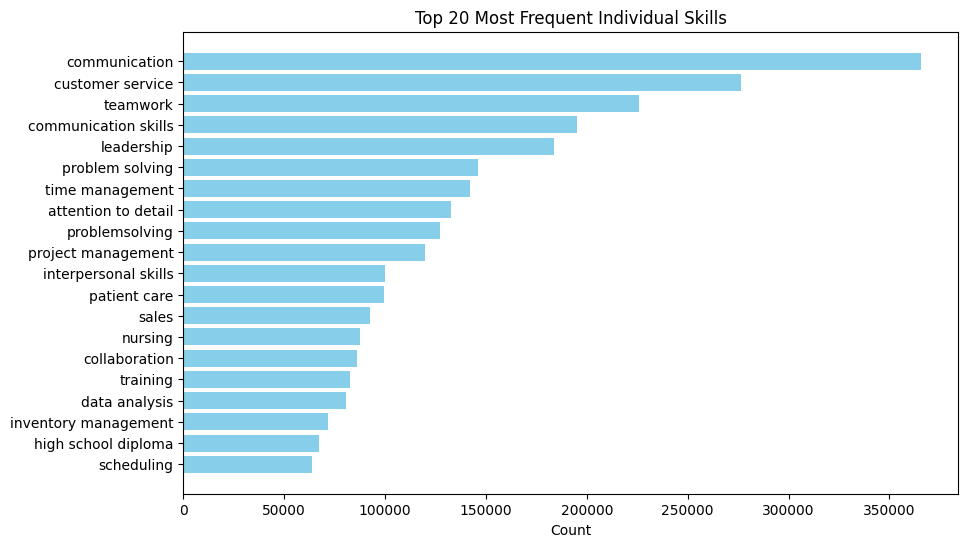
\includegraphics[width=0.9\linewidth]{download (23).png}
    \caption{Top 20 Most Frequent Individual Skills}
    \label{fig:singletons}
\end{figure}

\vspace{0.3cm}
Firstly, we analyze the 20 most frequent skills appearing in job postings. Unsurprisingly, the highest positions are taken by transversal soft skills like \textit{Communication}, \textit{Teamwork}, and \textit{Problem Solving}, underlining how social skills and the ability to work in a group are essential to any sector.
\textit{Data Analysis} is also present in the top 20, which suggests the growing importance of data-related skills across different sectors. 
Nursing and Patient Care also appear in the list, indicating a need for healthcare personnel.

\vspace{0.5cm}
\textbf{Overview of the Skill Pairs}

\vspace{0.3cm}
\begin{figure}[H]
    \centering
    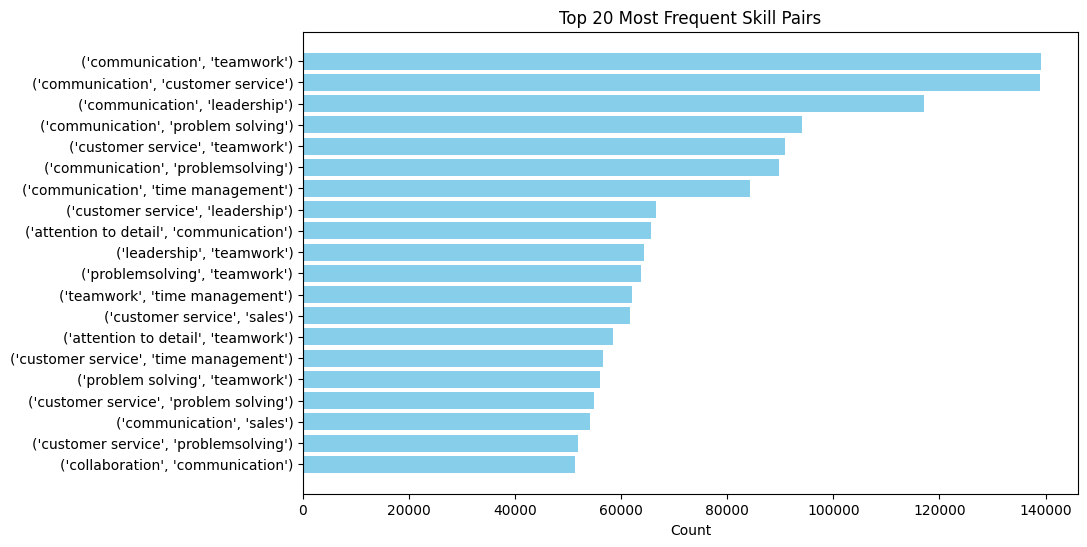
\includegraphics[width=0.9\linewidth]{download (24).png}
    \caption{Top 20 Most Frequent Skill Pairs}
    \label{fig:skill_pairs_1}
\end{figure}

\vspace{0.3cm}
\begin{figure}[H]
    \centering
    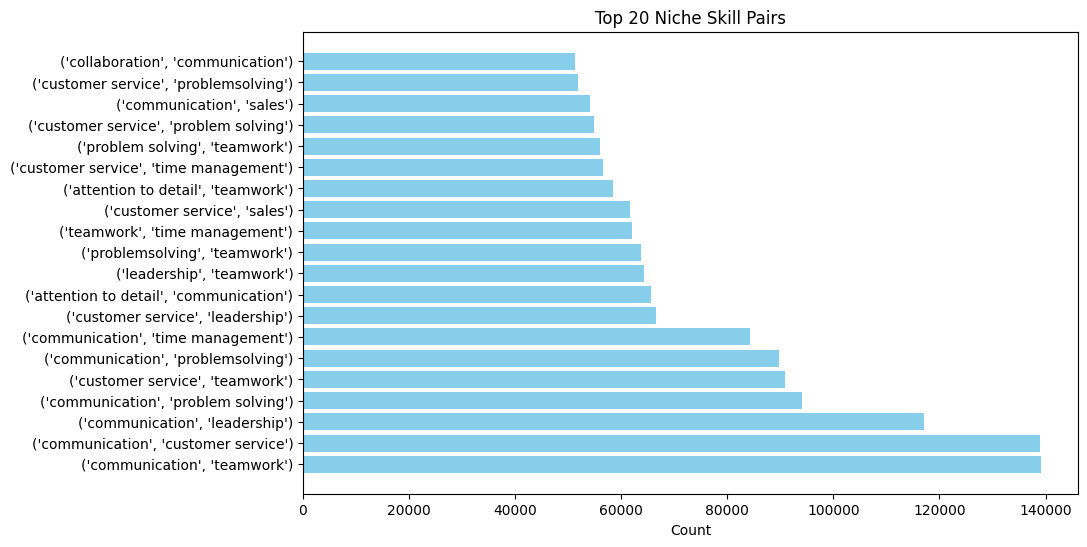
\includegraphics[width=0.9\linewidth]{download (25).png}
    \caption{Top 20 Niche Skill Pairs}
    \label{fig:skill_pairs_2}
\end{figure}

\vspace{0.3cm}
The overview of the frequently occurring pairs, determined by the Apriori algorithm, confirms the trend observed during the analysis of the singletons: the most sought-after skills are soft skills, specifically related to communicating to both colleagues and customers, as well as teamwork. This is evident in both the Top 20 most common pairs and the Top 20 niche pairs.

\vspace{0.5cm}
\textbf{Overview of the Skill Triplets}

\vspace{0.3cm}
\begin{figure}[H]
    \centering
    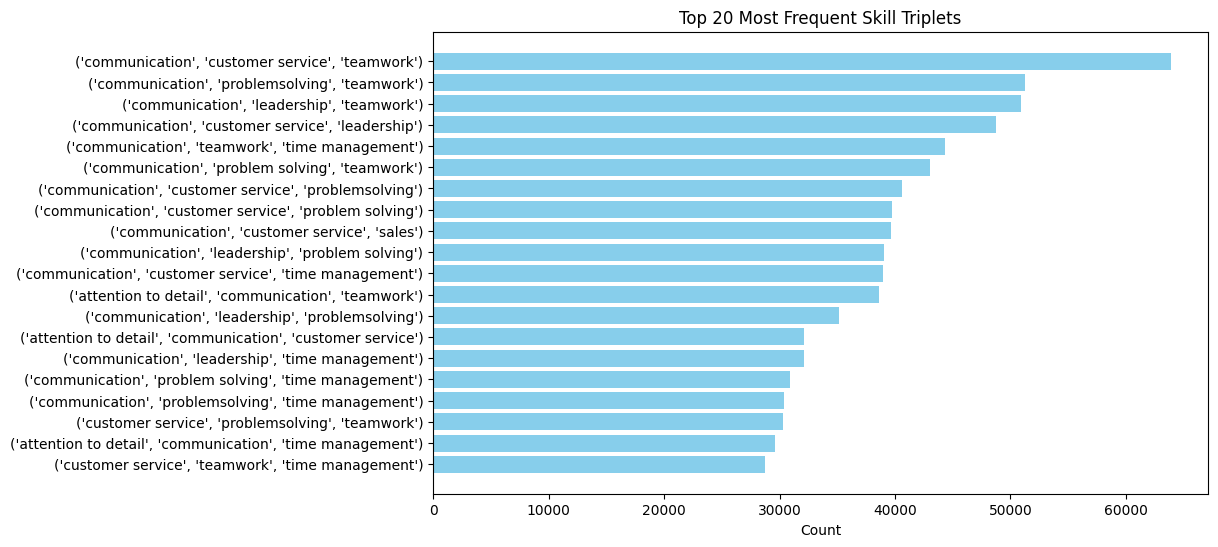
\includegraphics[width=0.9\linewidth]{download (26).png}
    \caption{Top 20 Most Frequent Skill Triplets}
    \label{fig:skill_triplets_1}
\end{figure}

\vspace{0.3cm}
\begin{figure}[H]
    \centering
    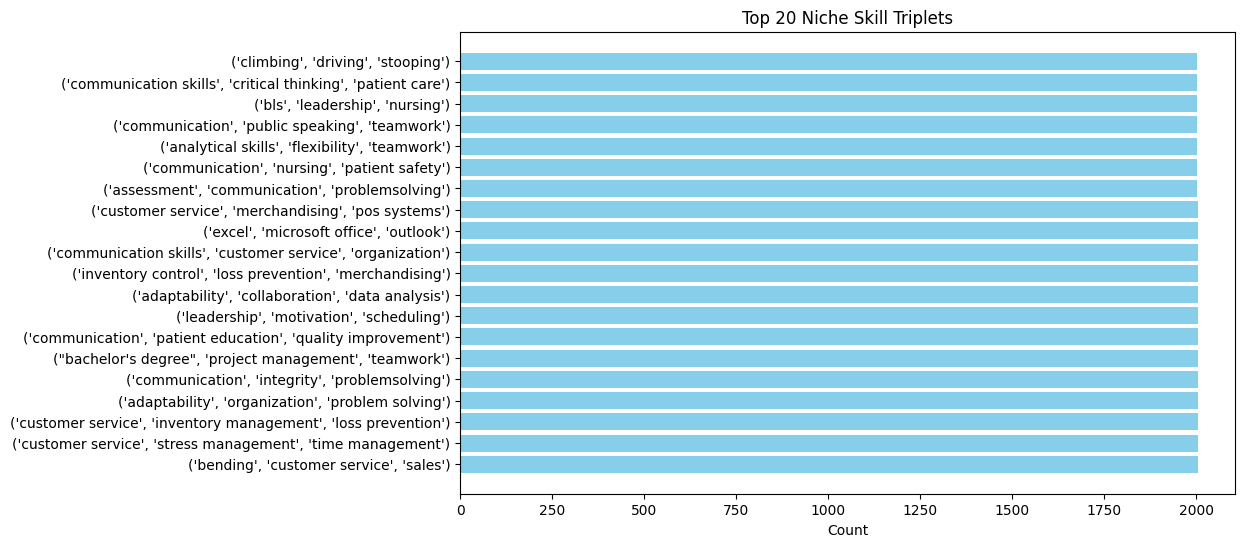
\includegraphics[width=0.9\linewidth]{download (27).png}
    \caption{Top 20 Niche Skill Triplets}
    \label{fig:skill_triplets_2}
\end{figure}

\vspace{0.3cm}
Similarly to the pairs, the most frequent triplets revolve around communication, customer service, and teamwork. These skills are highly valued across various job postings. 

However, the analysis of niche triplets highlights some specific demands:
\begin{itemize}
    \item \textbf{Climbing, Driving, Stooping}: This combination pertains to physical jobs, such as logistics or maintenance positions, where physical agility and strength are relevant.
    
    \item \textbf{Communication Skills, Critical Thinking, Patient Care}: This triplet suggests that in healthcare or service-related roles, being able to communicate effectively, think critically, and provide care to patients is highly valued.
    
    \item \textbf{Adaptability, Collaboration, Data Analysis}: This combination highlights the importance of flexibility in roles involving both teamwork and data analysis, possibly in dynamic business environments or research fields.
\end{itemize}



\section{FP-Growth Algorithm for Market Basket Analysis}
\subsection{FP-Growth Algorithm and computational demand of the Apriori Algorithm}

The FP-Growth (Frequent Pattern Growth) algorithm is an efficient alternative to the Apriori algorithm for identifying frequent itemsets in large datasets. Unlike Apriori, FP-Growth does not generate candidate itemsets. Instead, it uses a compressed data structure called the FP-Tree (Frequent Pattern Tree) to represent the dataset and recursively extracts frequent itemsets from this tree, which makes it faster and more scalable for large datasets.

One of the major drawbacks of the Apriori algorithm is its computational complexity, especially when dealing with large datasets and higher-order itemsets. As the number of itemsets grows, Apriori struggles to scale efficiently due to the generation of candidate itemsets at each iteration.

By implementing FP-Growth, we were able to explore higher-order itemsets to perform analysis which would be problematic to run using Apriori alone.


\subsection{Mathematical Framework}
Let $D$ represent a database of transactions, where each transaction contains a set of items from a universal set of items $I$. The FP-Growth algorithm aims to find frequent itemsets that meet a user-defined minimum support threshold, denoted by $\textit{min support}$.

\begin{itemize}
    \item \textbf{Itemset:} A set of one or more items from $I$.
    \item \textbf{Support:} The support of an itemset $X \subseteq I$ is defined as the proportion of transactions in the dataset $D$ in which the itemset $X$ appears. Mathematically:

\[
\text{Support}(X) = \frac{\text{Number of Transactions Containing } X}{\text{Total Number of Transactions}}
\]

    \item \textbf{Frequent Itemset:} An itemset $X$ is considered frequent if its support is greater than or equal to the minimum support threshold, i.e., $\text{Support}(X) \geq \textit{min support}$.
\end{itemize}

\subsection{Generating Frequent Itemsets}
FP-Growth leverages the FP-Tree, a compact representation of the dataset, which allows frequent itemsets to be generated without candidate generation. The key steps are as follows:

\subsection{Building the FP-Tree}
The FP-Growth algorithm starts by constructing a data structure known as the Frequent Pattern Tree (FP-Tree). The FP-Tree is a compressed representation of the transaction database that retains the frequency of individual items and the relationships between them. The construction of the FP-Tree involves several key steps:

\begin{enumerate}
    \item \textbf{First Database Scan:} The algorithm first scans the transaction database to identify frequent items. Items that do not meet the minimum support threshold are discarded at this stage. The remaining items are sorted in descending order of their frequency, which helps in building a compact and efficient FP-Tree.

    \item \textbf{Second Database Scan:} In the second scan, the algorithm processes each transaction in the dataset. For each transaction, it creates a path in the FP-Tree that links the items in the transaction. The items are added in the same frequency-based order determined in the first scan. If an item already exists in the current path, the algorithm increments the count of the existing node rather than creating a new node.

    \item \textbf{Shared Prefixes:} One of the key features of the FP-Tree is that transactions that share common items will share the same path in the tree. This sharing of paths leads to significant compression of the dataset, as common patterns are stored only once rather than being duplicated. For example, if multiple transactions include the itemset $\{A, B, C\}$, they will all follow the same path in the FP-Tree, with the counts of the nodes being incremented accordingly.

\end{enumerate}

\subsection{Recursive Pattern Growth}
Once the FP-Tree is built, the FP-Growth algorithm begins the process of mining frequent patterns. This is done recursively through the following steps:

\begin{enumerate}
    \item \textbf{Mining Frequent Patterns:} Starting from the least frequent item in the header table, the algorithm traces all paths in the FP-Tree where this item appears. These paths are used to construct a conditional pattern base, which is essentially a subset of transactions that co-occur with the item. Based on this pattern base, a conditional FP-Tree is built.

    \item \textbf{Recursive Mining:} The algorithm recursively mines each conditional FP-Tree to extract frequent itemsets. For each conditional FP-Tree, new frequent itemsets are found, and the process continues until no more frequent patterns can be extracted from the tree.

    \item \textbf{Efficiency Gains:} By using conditional FP-Trees, FP-Growth avoids generating and testing candidate itemsets. The recursive nature of the algorithm allows it to focus on smaller subsets of the dataset in each iteration, which makes it significantly more efficient than Apriori for large datasets.
\end{enumerate}

In fact, unlike the Apriori algorithm, which generates candidate itemsets and performs multiple scans of the database, FP-Growth compresses the dataset into an FP-Tree and performs a recursive search for frequent patterns. This reduces the computational cost and time, especially for large datasets.

\subsection{Application of FP-Growth Algorithm}
Implementation:
\begin{enumerate}
    \item \textbf{Data Preparation:} Clean and preprocess the dataset.
    \item \textbf{Apply FP-Growth:} Construct the FP-Tree and recursively extract frequent itemsets using the FP-Growth algorithm.
\end{enumerate}

\subsection{Findings}

\vspace{0.5cm}
\textbf{Overview of the Skill Quadruplets}

\vspace{0.3cm}
\begin{figure}[H]
    \centering
    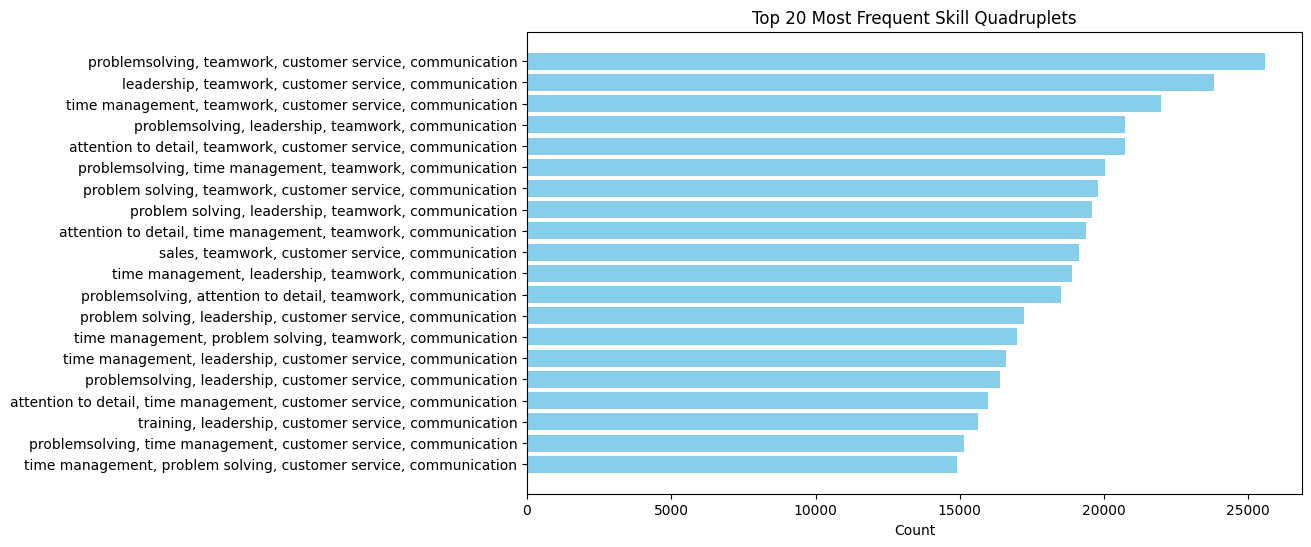
\includegraphics[width=1\linewidth]{download (28).png}
    \caption{Top 20 Most Frequent Skill Quadruplets}
    \label{fig:skill_pairs_1}
\end{figure}

\vspace{0.3cm}
\begin{figure}[H]
    \centering
    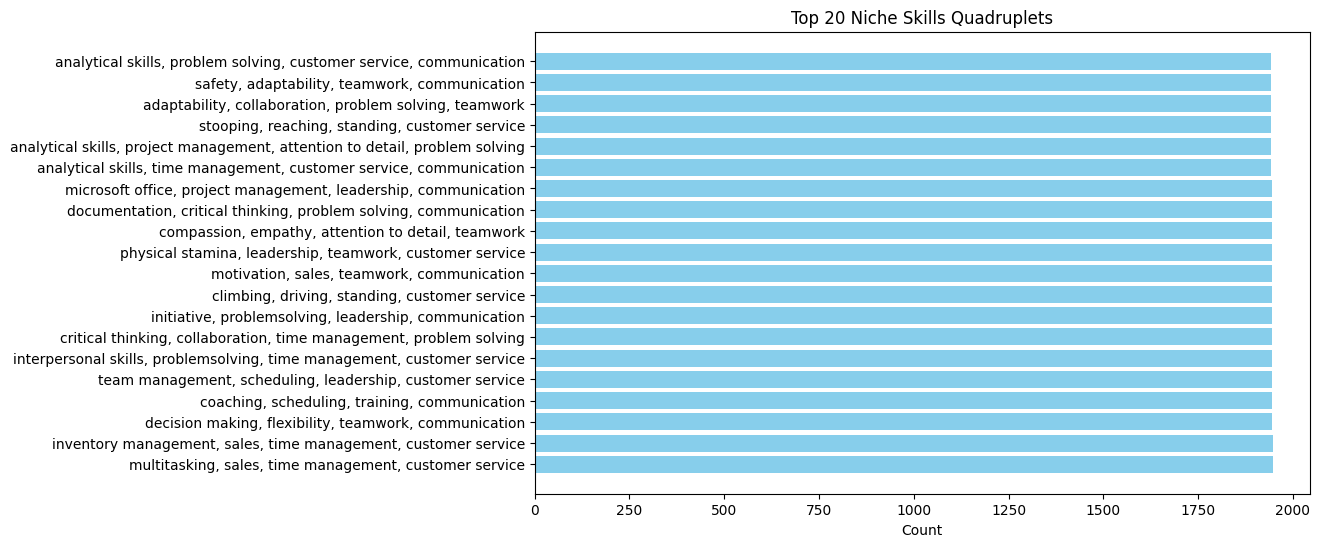
\includegraphics[width=1\linewidth]{download (29).png}
    \caption{Top 20 Niche Skill Quadruplets}
    \label{fig:skill_pairs_2}
\end{figure}

\vspace{0.3cm}
Not surprisingly, the overview of the quadruplets, emphasizes soft skills, with communication, teamwork, customer service, and problem-solving being the most frequent skills that appear in various combinations
The chart depicting the Top 20 Niche Quadruplets however, hints at more specific roles that are sought after:

\begin{itemize}
    \item \textbf{Analytical Skills, Problem Solving, Customer Service, Communication}: 
    This combination suggests roles that require both analytical thinking and the ability to effectively communicate with clients.

    \item \textbf{Safety, Adaptability, Teamwork, Communication}: 
    This combination could point to safety-critical industries, and offers an overview of the skillsets that is sought after.

    \item \textbf{Climbing, Driving, Standing, Customer Service}: 
    This indicates a niche demand for roles that require physical stamina and skills, possibly in sectors like logistics, maintenance, or outdoor services, where interaction with customers is also expected.
\end{itemize}

\vspace{0.5cm}
\textbf{Overview of the Skill Quintuplets}

\vspace{0.3cm}
\begin{figure}[H]
    \centering
    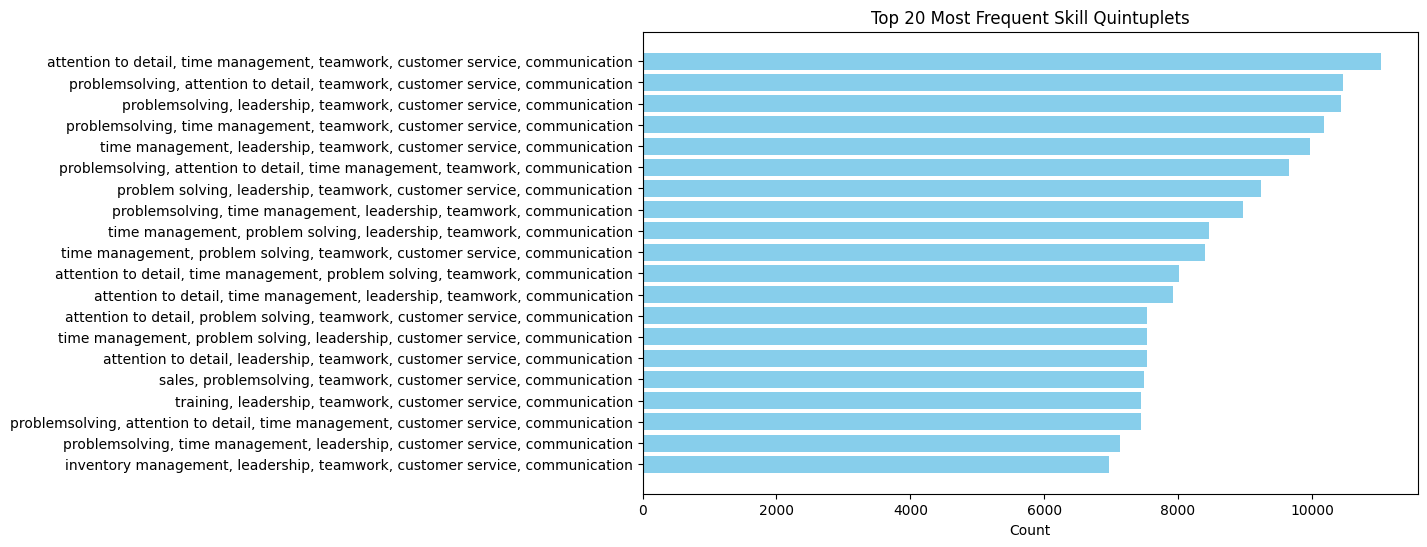
\includegraphics[width=1\linewidth]{download (30).png}
    \caption{Top 20 Most Frequent Skill Quintuplets}
    \label{fig:skill_pairs_1}
\end{figure}

\vspace{0.3cm}
\begin{figure}[H]
    \centering
    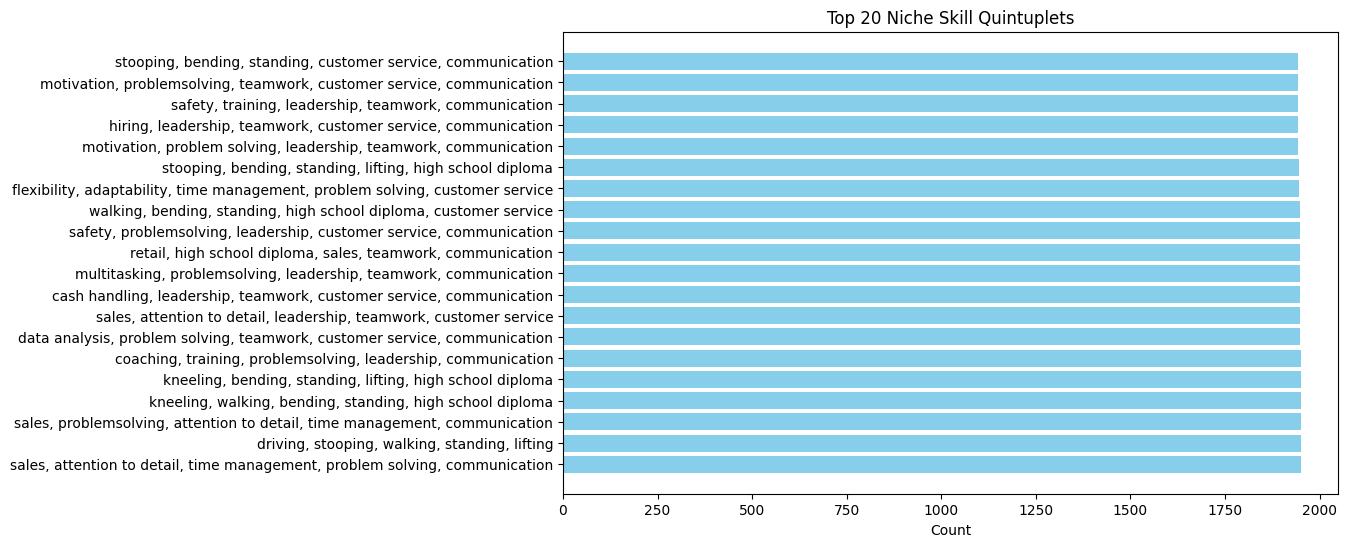
\includegraphics[width=1\linewidth]{download (31).png}
    \caption{Top 20 Niche Skill Quintuplets}
    \label{fig:skill_pairs_2}
\end{figure}

\vspace{0.3cm}
The Top 20 Most Frequent Quintuplets generated by the FP-Growth algorithm again reveal a tendency for employee to directly search for a wide range of soft skills related to the social and communicative sphere. The overview of the niche quintuplets, however, offers some insight regarding unique combinations of skills:

\begin{itemize}
    \item \textbf{Stooping, Bending, Standing, Customer Service, Communication}: 
    This quintuplet likely refers to physical demanding jobs where constant movement is required, as well as interacting with customers, for example retail or logistics.

    \item \textbf{Data Analysis, Problem Solving, Teamwork, Customer Service, Communication}: 
    This combination highlights how, in Data Analytics positions, it is important to work in a team and have good communicative skills with customers.

\end{itemize}

\vspace{0.5cm}
\textbf{Absence of Skill Sextuplets}

\vspace{0.3cm}

The FP-Growth algorithm did not identify any sextuplet with frequency above support. This suggests that job postings focus on a limited set of skills, which, by our analysis, mostly concern transversal soft skills which are required at any level. Quintuplets provide an extensive view of what companies are looking for, and any additional skill would not be adding value to job postings.

\newpage
\section{Conclusion: An Overview of Data Analytics Job Offerings}

In the concluding phase of our market-basket analysis, we focused on job skills related to the field of data analytics. The analysis was performed using the FP-Growth algorithm. We will be focusing on the most relevant pairs and quintuplets containing target skills related to data analysis, data science, and machine learning.

\subsection{Focus on Pairs}

\vspace{0.3cm}
\begin{figure}[H]
    \centering
    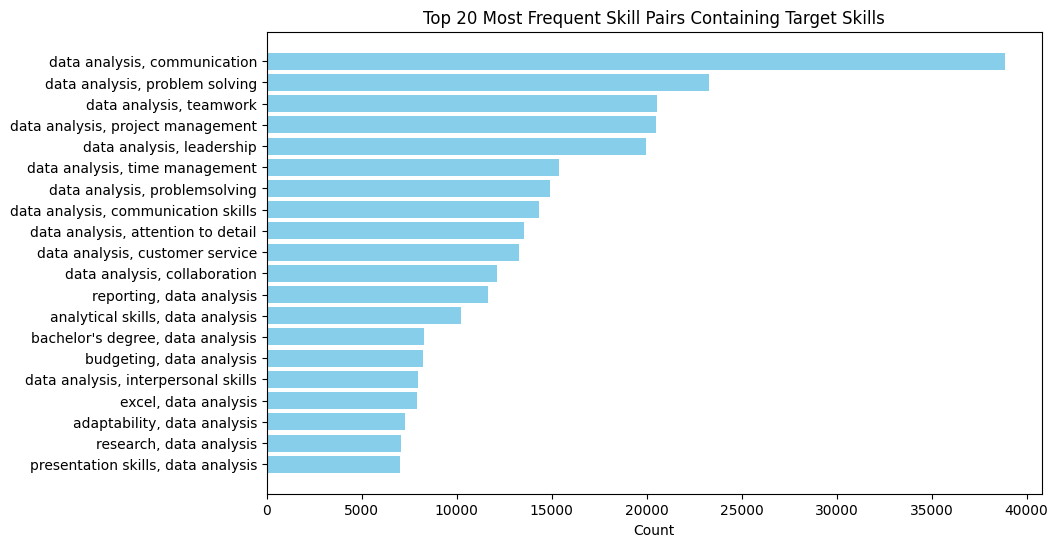
\includegraphics[width=1\linewidth]{download (36).png}
    \caption{Top 20 Most Frequent Data Related Pairs}
    \label{fig:skill_pairs_1}
\end{figure}


The overview of pairs provided significant insights into the most common skill combinations in the field of data analytics. The top pairs highlight how skills pertaining to the social sphere are sought after: it may indicate the relevancy of analyzing data and communicating the outcomes to external non-technical stakeholders.
These pairs underline the multidisciplinary nature of roles in data analytics, where technical skills are equally as important as soft skills such as leadership and problem-solving abilities. 
Data Analytics offerings are also often paired with the requirement of having a Bachelor's Degree, defining how a higher education is necessary for the more technical skills.



\subsection{Focus on Quintuplets}

\vspace{0.3cm}
\begin{figure}[H]
    \centering
    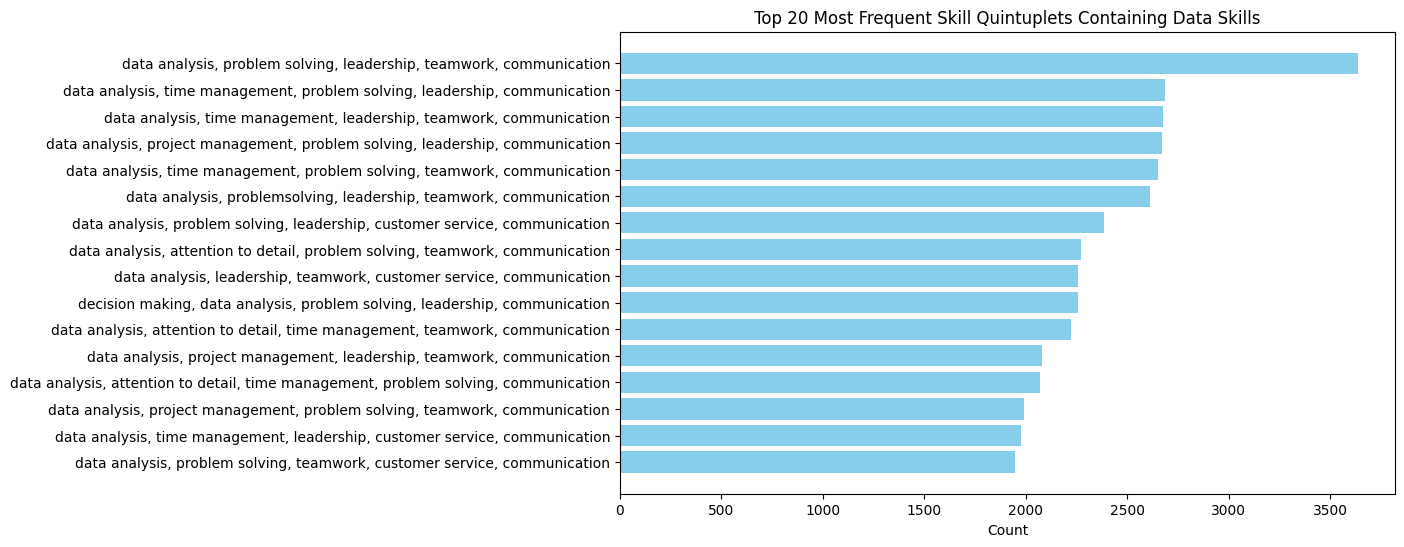
\includegraphics[width=1\linewidth]{download (37).png}
    \caption{Top 20 Most Frequent Data Related Quintuplets}
    \label{fig:skill_pairs_1}
\end{figure}

The exploration of quintuplets provide a more generic overview of the Data Analytics postings, once again underlining how a specific set of social transversal skills is relevant, perhaps for better communication with customers and stake holders.
A focus on project management and leadership is also evident, highlighting how the ability of managing large scale projects is sought after by employees.

\newpage

I/We declare that this material, which I/We now submit for assessment, is entirely my/our own work and has not been taken from the work of others, save and to the extent that such work has been cited and acknowledged within the text of my/our work, and including any code produced using generative AI systems. I/We understand that plagiarism, collusion, and copying are grave and serious offences in the university and accept the penalties that would be imposed should I engage in plagiarism, collusion or copying. This assignment, or any part of it, has not been previously submitted by me/us or any other person for assessment on this or any other course of study.
\end{document}
